\documentclass[../../Orator.tex]{subfiles}

\begin{document}





% This figure should point to Scale of models
\begin{figure}[ht]
    \centering
    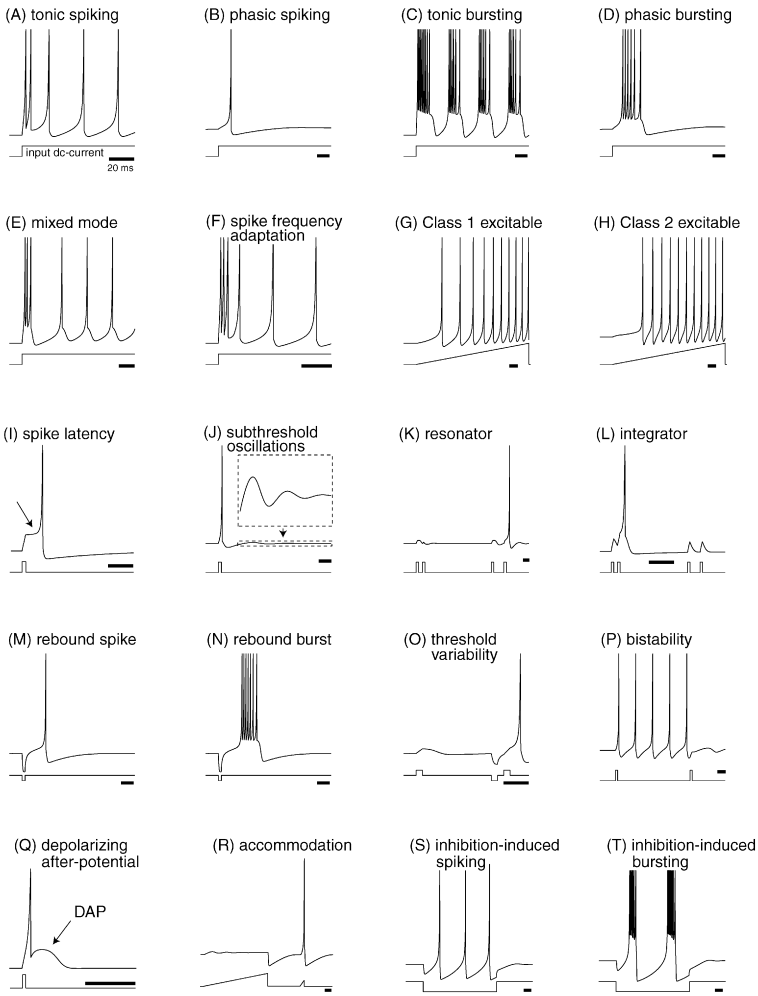
\includegraphics{Pictures/Kenni/Summary biological spiking neurons.png}
    \caption{Summary of the neuro-computational properties of biological spiking neurons. Shown are simulations of the same model (1) and (2), with different choices
    of parameters. Each horizontal bar denotes a 20-ms time interval, ~\cite{izhikevich2004model}}
    \label{fig:sum_spike_neuro}
\end{figure}
 
 NEURO-COMPUTATIONAL FEATURES:
 This figure shows 20 of the most prominent features of biological spiking neurons and depicts the spiking behavior of individual neurons in response to simple pulses of dc current, ~\cite{izhikevich2004model}.















\end{document}